\documentclass[12pt]{article}
\usepackage[a4paper, left=5mm, right=5mm, top=5mm, bottom=5mm]{geometry}
\usepackage[russian]{babel}
\usepackage{fontspec}
\usepackage{graphicx}
\usepackage[unicode]{hyperref}
\usepackage{enumitem}
\usepackage{wrapfig}
\usepackage{tabularx}
\usepackage{amssymb}
\usepackage{gensymb}
\usepackage{amsmath}
\usepackage{blindtext}
\usepackage{float}
\usepackage{multicol}
\usepackage{latexsym}
\usepackage{caption}
\usepackage{subcaption}
\usepackage{listings}
\usepackage{xcolor}
\usepackage{breqn}
\usepackage{pdfpages}
\usepackage{forest}
\useforestlibrary{linguistics} 

\setmainfont{Times New Roman}
\setmonofont{Courier New}
\righthyphenmin=2 % правильные переносы
\graphicspath{{images/}} % путь к картинкам

\forestapplylibrarydefaults{linguistics}
\newcommand{\teta}{\vartriangleright\!\vartriangleleft} %тета соединение

\title{Lab7 BD}
\author{Азат Сиразетдинов}

\begin{document}
	{\thispagestyle{empty}
	\begin{center}
		Федеральное государственное автономное образовательное учреждение\\ 
		высшего образования\\
		«Национальный исследовательский университет ИТМО»\\
		\textit{Факультет Программной Инженерии и Компьютерной Техники}\\
	\end{center}
	\vspace{2cm}
	\begin{center}
		\large
		\textbf{Лабораторная работа № 4}\\
		по дисциплине базы данных\\
		Индексы\\
		Вариант № 1678
	\end{center}
	\vspace{7cm}
	\begin{flushright}
		Выполнил:\\
		cтудент  группы P3116\\
		Сиразетдинов А. Н\\
		Преподаватель: \\
		Горбунов М. В.\\
	\end{flushright}
	\vspace{6cm}
	\begin{center}
		г. Санкт-Петербург\\
		2023г.
	\end{center}
	\newpage
	}
	\tableofcontents
	\newpage
	
	\section{Текст задания}
	Составить запросы на языке SQL (пункты 1-2).
	
	Для каждого запроса предложить индексы, добавление которых уменьшит время выполнения запроса (указать таблицы/атрибуты, для которых нужно добавить индексы, написать тип индекса; объяснить, почему добавление индекса будет полезным для данного запроса).
	
	Для запросов 1-2 необходимо составить возможные планы выполнения запросов. Планы составляются на основании предположения, что в таблицах отсутствуют индексы. Из составленных планов необходимо выбрать оптимальный и объяснить свой выбор.
	Изменятся ли планы при добавлении индекса и как?
	
	Для запросов 1-2 необходимо добавить в отчет вывод команды EXPLAIN ANALYZE [запрос]
	
	Подробные ответы на все вышеперечисленные вопросы должны присутствовать в отчете (планы выполнения запросов должны быть нарисованы, ответы на вопросы - представлены в текстовом виде).
	
	Сделать запрос для получения атрибутов из указанных таблиц, применив фильтры по указанным условиям:
	
	Н_ТИПЫ_ВЕДОМОСТЕЙ, Н_ВЕДОМОСТИ.
	
	Вывести атрибуты: Н_ТИПЫ_ВЕДОМОСТЕЙ.ИД, Н_ВЕДОМОСТИ.ЧЛВК_ИД.
	
	Фильтры (AND):
	\begin{enumerate}[]
	\item Н_ТИПЫ_ВЕДОМОСТЕЙ.НАИМЕНОВАНИЕ > Ведомость.
	\item Н_ВЕДОМОСТИ.ИД > 1250981.
	\end{enumerate}
	Вид соединения: RIGHT JOIN.
	
	Сделать запрос для получения атрибутов из указанных таблиц, применив фильтры по указанным условиям:
	
	Таблицы: Н_ЛЮДИ, Н_ОБУЧЕНИЯ, Н_УЧЕНИКИ.
	
	Вывести атрибуты: Н_ЛЮДИ.ИМЯ, Н_ОБУЧЕНИЯ.ЧЛВК_ИД, Н_УЧЕНИКИ.НАЧАЛО.
	
	Фильтры: (AND)
	\begin{enumerate}[]
	\item Н_ЛЮДИ.ФАМИЛИЯ < Ёлкин.
	\item Н_ОБУЧЕНИЯ.ЧЛВК_ИД > 112514.
	\item Н_УЧЕНИКИ.ИД > 100410.
	\end{enumerate}
	Вид соединения: RIGHT JOIN.
	\newpage
	
	\section{Запрос 1}
	\subsection{Реализация запроса на SQL}
	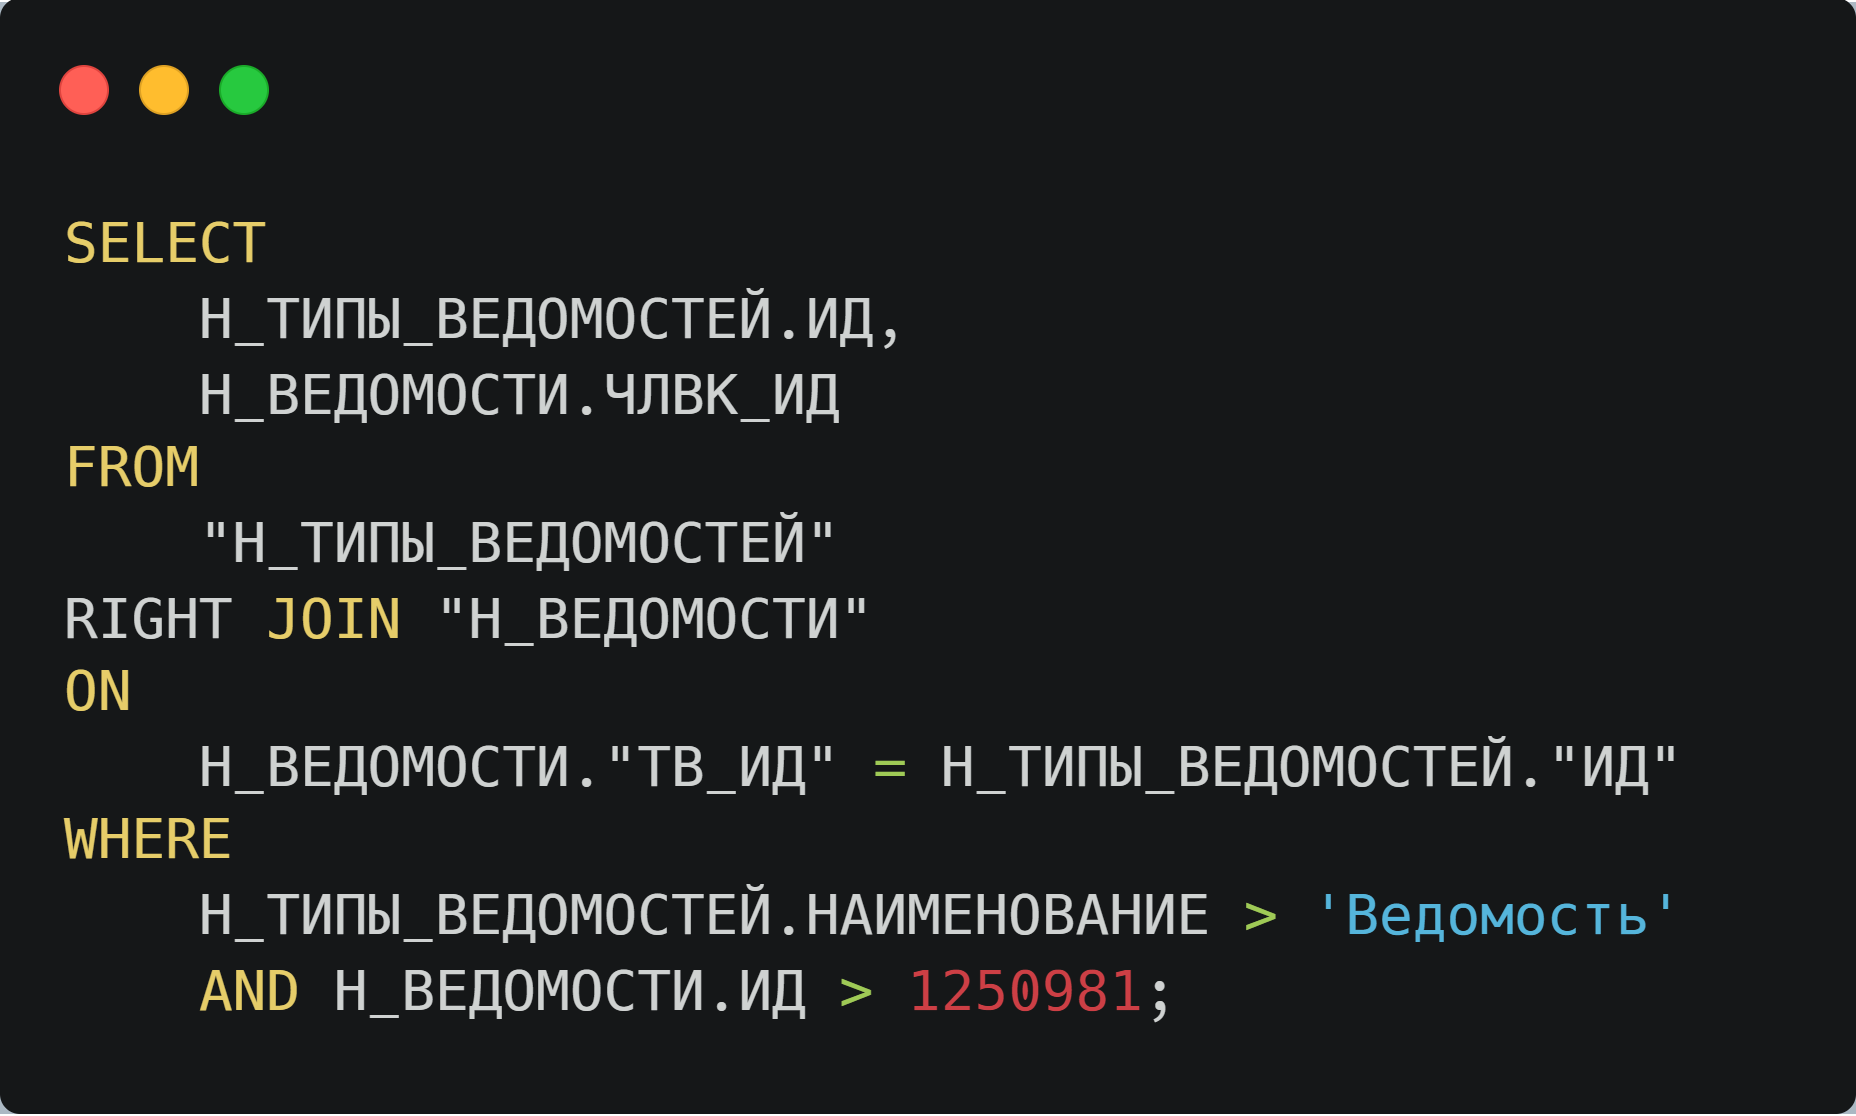
\includegraphics[width=0.5\linewidth]{sql1}
	\subsection{Использование индексов}
	\subsubsection*{Таблица \texttt{Н_ТИПЫ_ВЕДОМОСТЕЙ}}
	
	Индекс b-tree на атрибуте \texttt{НАИМЕНОВАНИЕ} уменьшит время выполнения запроса, потому что индекс b-tree хорошо подходит для операций выборок больше определенного значения
	\subsubsection*{Таблица \texttt{Н_ВЕДОМОСТИ}}
	
	Индекс b-tree на атрибуте \texttt{ИД} уменьшит время выполнения запроса, потому что индекс b-tree хорошо подходит для операций выборок больше определенного значения
	
	\subsection{Планы выполнения запроса}
	\subsubsection*{План 1}
	\begin{forest}
	 /tikz/every node/.append style={font=\large},
	[$\pi_{\text{Н_ТИПЫ_ВЕДОМОСТЕЙ.ЧЛВК_ИД, Н_ВЕДОМОСТИ.ЧЛВК_ИД}}$
		[$\sigma_{\text{Н_ТИПЫ_ВЕДОМОСТЕЙ.НАИМЕНОВАНИЕ}}$
			[$\sigma_{\text{Н_ВЕДОМОСТИ.ИД}}$
				[$\teta_{\text{Н_ТИПЫ_ВЕДОМОСТЕЙ.ИД=Н_ВЕДОМОСТИ.ТВ_ИД}}$
					[Н_ТИПЫ_ВЕДОМОСТЕЙ]
					[Н_ВЕДОМОСТИ]
				]
			]
		]
	]
	\end{forest}
	\subsubsection*{План 2}
	\begin{forest}
		/tikz/every node/.append style={font=\large},
		[$\pi_{\text{Н_ТИПЫ_ВЕДОМОСТЕЙ.ЧЛВК_ИД, Н_ВЕДОМОСТИ.ЧЛВК_ИД}}$
			[$\sigma_{\text{Н_ВЕДОМОСТИ.ИД}}$
				[$\teta_{\text{Н_ТИПЫ_ВЕДОМОСТЕЙ.ИД=Н_ВЕДОМОСТИ.ТВ_ИД}}$
					[$\sigma_{\text{Н_ТИПЫ_ВЕДОМОСТЕЙ.НАИМЕНОВАНИЕ}}$
						[Н_ТИПЫ_ВЕДОМОСТЕЙ]]
					[Н_ВЕДОМОСТИ]
				]
			]
		]
	\end{forest}
	\subsubsection*{План 3}
	\begin{forest}
		/tikz/every node/.append style={font=\large},
		[$\pi_{\text{Н_ТИПЫ_ВЕДОМОСТЕЙ.ЧЛВК_ИД, Н_ВЕДОМОСТИ.ЧЛВК_ИД}}$
			[$\sigma_{\text{Н_ВЕДОМОСТИ.ИД}}$
				[$\teta_{\text{Н_ТИПЫ_ВЕДОМОСТЕЙ.ИД=Н_ВЕДОМОСТИ.ТВ_ИД}}$
					[$\sigma_{\text{Н_ТИПЫ_ВЕДОМОСТЕЙ.НАИМЕНОВАНИЕ}}$
						[$\pi_{\text{НАИМЕНОВАНИЕ, ИД, ЧЛВК_ИД}}$
							[Н_ТИПЫ_ВЕДОМОСТЕЙ]
						]
					]
					[Н_ВЕДОМОСТИ]
				]
			]
		]
	\end{forest}
	\subsubsection*{План 4}
	\begin{forest}
		/tikz/every node/.append style={font=\large},
		[$\pi_{\text{Н_ТИПЫ_ВЕДОМОСТЕЙ.ЧЛВК_ИД, Н_ВЕДОМОСТИ.ЧЛВК_ИД}}$
			[$\sigma_{\text{Н_ВЕДОМОСТИ.ИД}}$
				[$\teta_{\text{Н_ТИПЫ_ВЕДОМОСТЕЙ.ИД=Н_ВЕДОМОСТИ.ТВ_ИД}}$
					[$\sigma_{\text{Н_ТИПЫ_ВЕДОМОСТЕЙ.НАИМЕНОВАНИЕ}}$
						[$\pi_{\text{НАИМЕНОВАНИЕ, ИД, ЧЛВК_ИД}}$
							[Н_ТИПЫ_ВЕДОМОСТЕЙ]
						]
					]
					[$\pi_{\text{ТВ_ИД, ИД, ЧЛВК_ИД}}$
						[Н_ВЕДОМОСТИ]
					]
				]
			]
		]
	\end{forest}
	\subsubsection*{План 5}
	\begin{forest}
		/tikz/every node/.append style={font=\large},
		[$\pi_{\text{Н_ТИПЫ_ВЕДОМОСТЕЙ.ЧЛВК_ИД, Н_ВЕДОМОСТИ.ЧЛВК_ИД}}$
			[$\teta_{\text{Н_ТИПЫ_ВЕДОМОСТЕЙ.ИД=Н_ВЕДОМОСТИ.ТВ_ИД}}$
				[$\sigma_{\text{Н_ВЕДОМОСТИ.ИД}}$
					[Н_ВЕДОМОСТИ]
				]
				[$\sigma_{\text{Н_ТИПЫ_ВЕДОМОСТЕЙ.НАИМЕНОВАНИЕ}}$
					[Н_ТИПЫ_ВЕДОМОСТЕЙ]
				]
			]
		]
	\end{forest}
	\subsubsection*{План 6}
	\begin{forest}
		/tikz/every node/.append style={font=\large},
		[$\pi_{\text{Н_ТИПЫ_ВЕДОМОСТЕЙ.ЧЛВК_ИД, Н_ВЕДОМОСТИ.ЧЛВК_ИД}}$
			[$\teta_{\text{Н_ТИПЫ_ВЕДОМОСТЕЙ.ИД=Н_ВЕДОМОСТИ.ТВ_ИД}}$
				[$\sigma_{\text{Н_ВЕДОМОСТИ.ИД}}$
					[$\pi_{\text{ИД, ЧЛВК_ИД, ТВ_ИД}}$
						[Н_ВЕДОМОСТИ]
					]
				]
				[$\sigma_{\text{Н_ТИПЫ_ВЕДОМОСТЕЙ.НАИМЕНОВАНИЕ}}$
					[$\pi_{\text{НАИМЕНОВАНИЕ, ИД, ЧЛВК_ИД}}$
						[Н_ТИПЫ_ВЕДОМОСТЕЙ]
					]
				]
			]
		]
	\end{forest}
	
	\subsection{Оптимальный план}

	Самый оптимальный план - План 6, потому что он использует левостороннее дерево и все выборки и проекции сделаны максимально рано.
	
	\subsection{Выполнение команды \texttt{EXPLAIN ANALYZE}}
	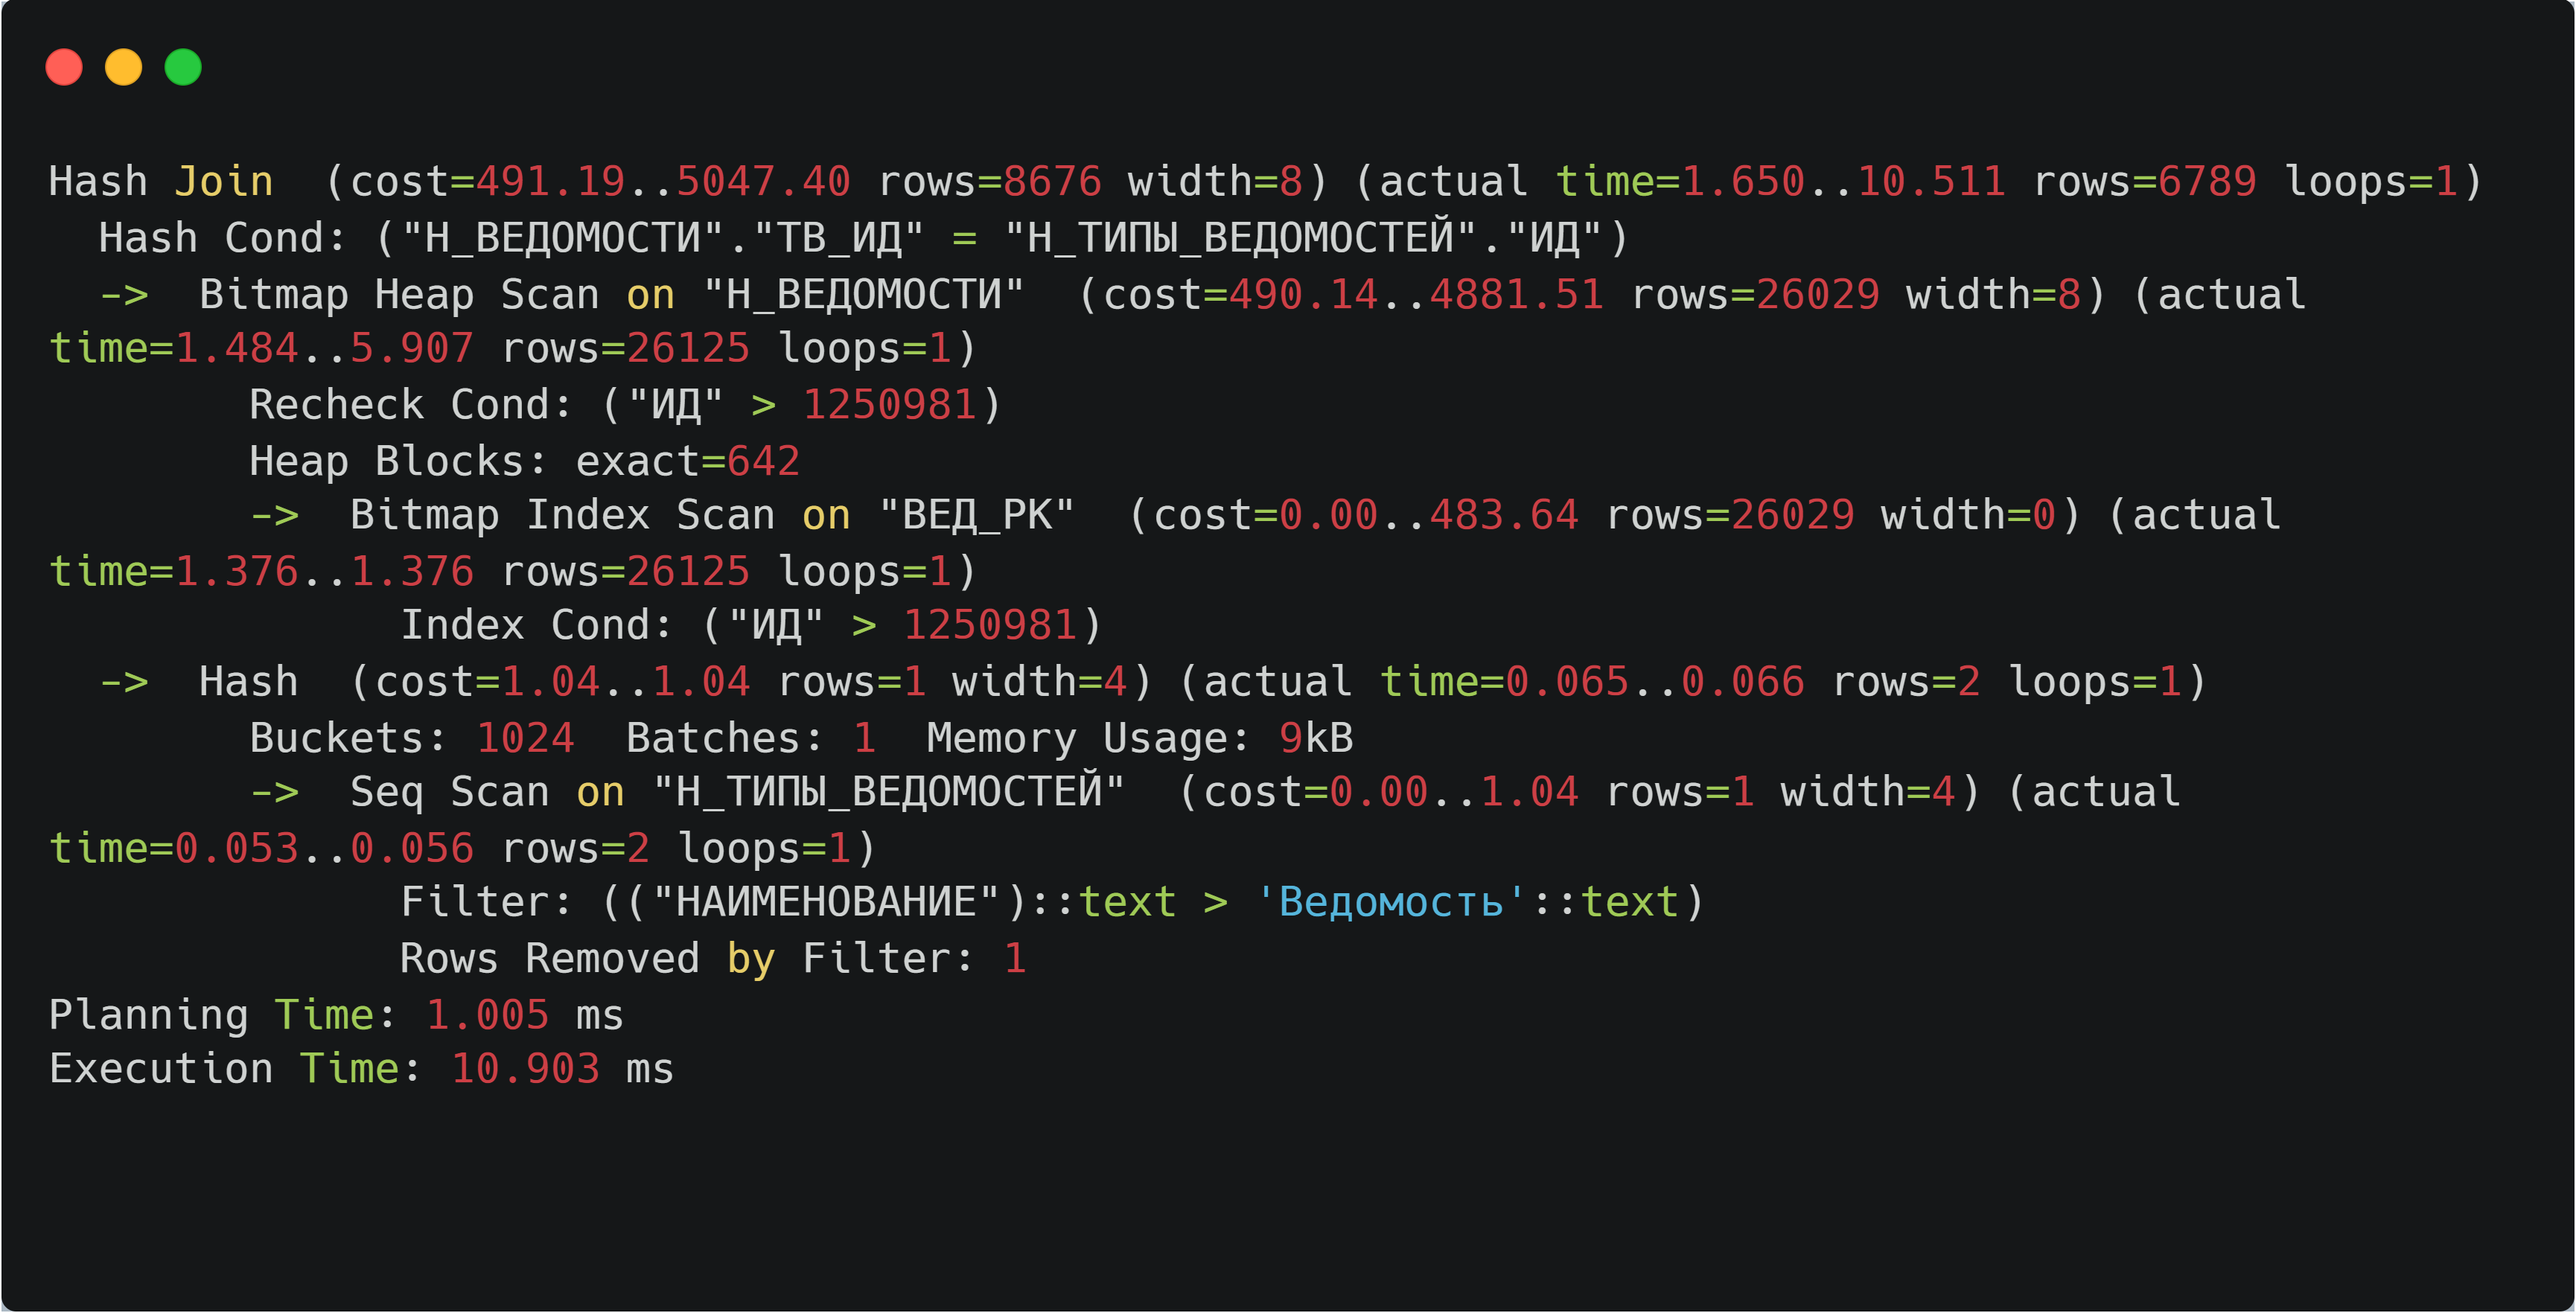
\includegraphics[width=\linewidth]{explain1}
	\newpage
	
	\section{Запрос 2}
	\subsection{Реализация запроса на SQL}
	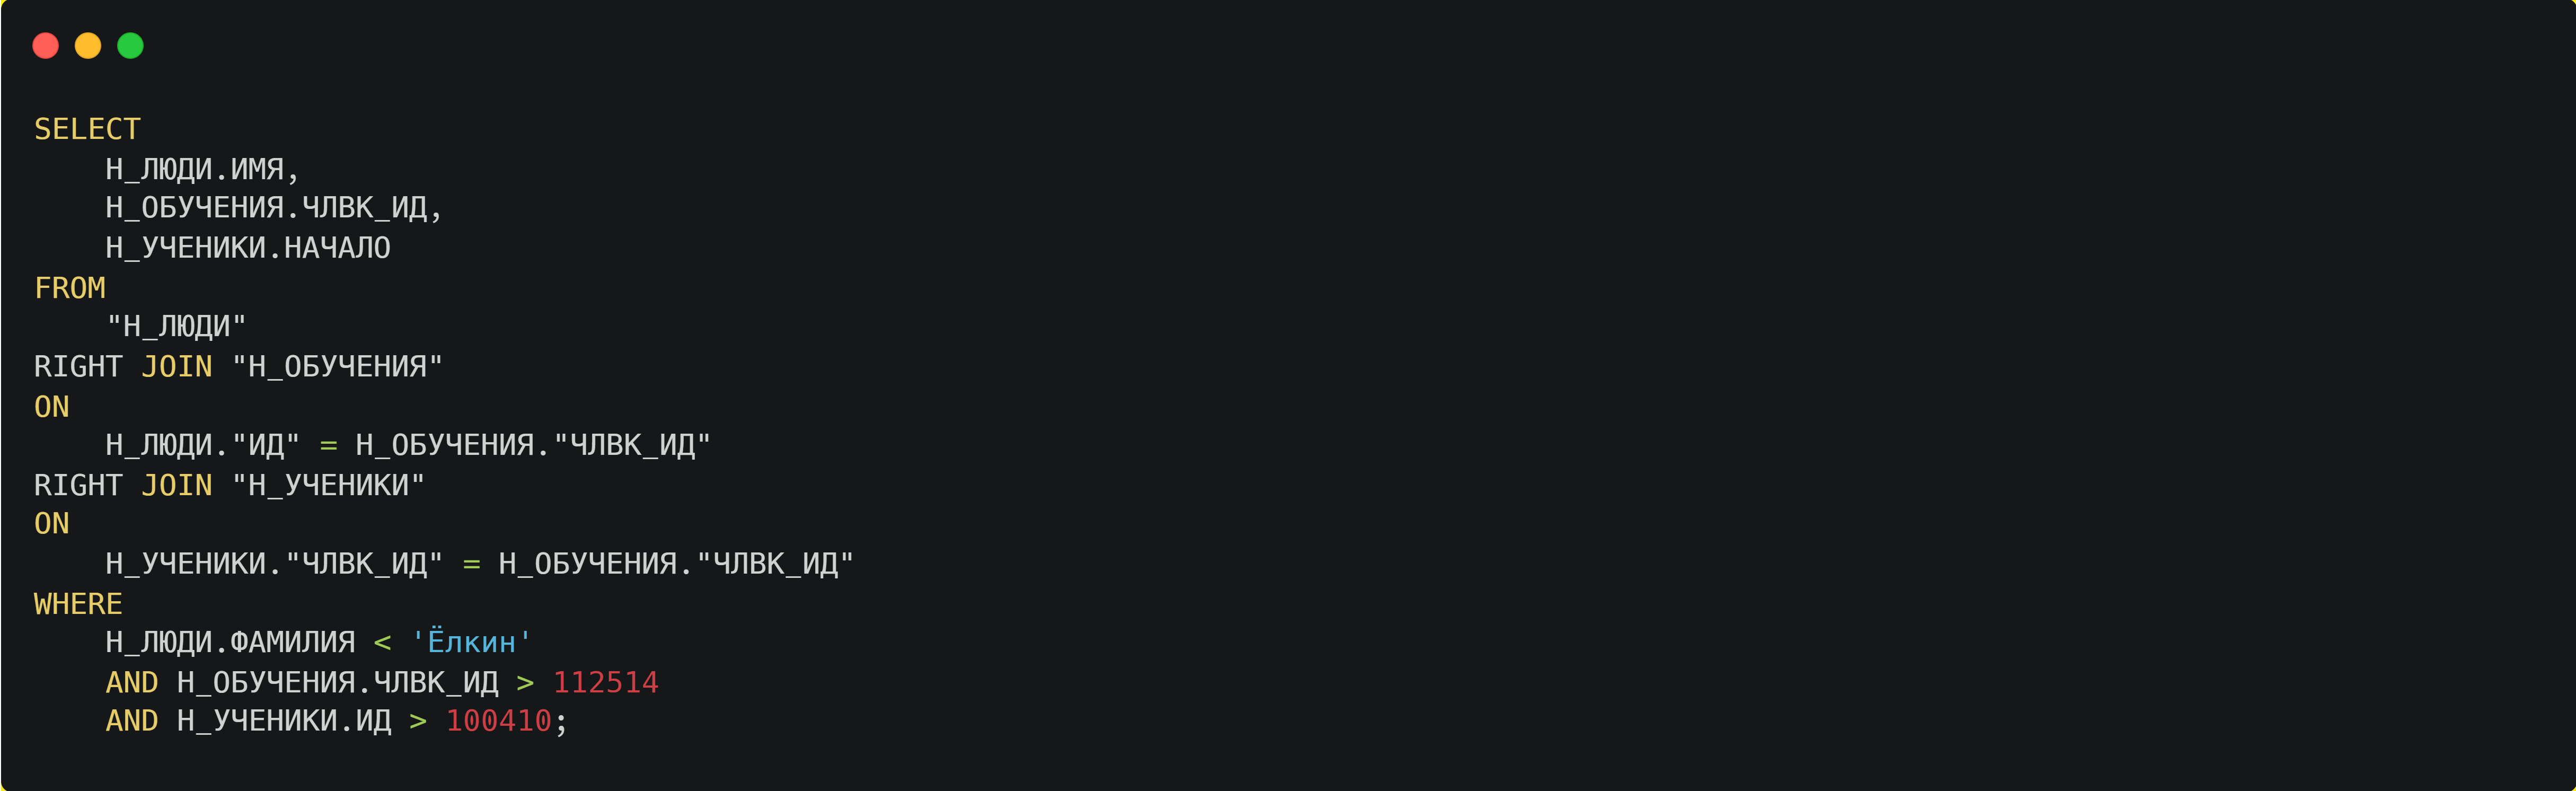
\includegraphics[width=0.5\linewidth]{images/sql2}
	
	\subsection{Использование индексов}

	\subsubsection*{Таблица \texttt{Н_ЛЮДИ}}
	
	Индекс b-tree на атрибуте \texttt{ФАМИЛИЯ} уменьшит время выполнения запроса, потому что индекс b-tree хорошо подходит для операций выборок меньше определенного значения
	\subsubsection*{Таблица \texttt{Н_ОБУЧЕНИЯ}}
	
	Индекс b-tree на атрибуте \texttt{ЧЛВК_ИД} уменьшит время выполнения запроса, потому что индекс b-tree хорошо подходит для операций выборок больше определенного значения
	\subsubsection*{Таблица \texttt{Н_УЧЕНИКИ}}
	
	Индекс b-tree на атрибуте \texttt{ИД} уменьшит время выполнения запроса, потому что индекс b-tree хорошо подходит для операций выборок больше определенного значения
	
	\subsection{Планы выполнения запросов}
	\subsubsection*{План 1}
	\begin{forest}
		/tikz/every node/.append style={font=\large},
		[$\pi_{\text{Н_ЛЮДИ.ИМЯ, Н_ОБУЧЕНИЯ.ЧЛВК_ИД, Н_УЧЕНИКИ.НАЧАЛО}}$
			[$\sigma_{\text{Н_ЛЮДИ.ФАМИЛИЯ}}$
				[$\sigma_{\text{Н_ОБУЧЕНИЯ.ЧЛВК_ИД}}$
					[$\sigma_{\text{Н_УЧЕНИКИ.ИД}}$
						[$\teta_{\text{Н_УЧЕНИКИ.ЧЛВК_ИД = Н_ОБУЧЕНИЯ.ЧЛВК_ИД ^ Н_УЧЕНИКИ.ВИД_ОБУЧ_ИД = Н_ОБУЧЕНИЯ.ВИД_ОБУЧ_ИД}}$
							[$\teta_{\text{Н_ЛЮДИ.ИД = Н_ОБУЧЕНИЯ.ЧЛВК_ИД}}$
								[Н_ЛЮДИ]
								[Н_ОБУЧЕНИЯ]
							]
							[Н_УЧЕНИКИ]
						]
					]
				]
			]
		]
	\end{forest}
	\subsubsection*{План 2}
	\begin{forest}
		/tikz/every node/.append style={font=\large},
		[$\pi_{\text{Н_ЛЮДИ.ИМЯ, Н_ОБУЧЕНИЯ.ЧЛВК_ИД, Н_УЧЕНИКИ.НАЧАЛО}}$
			[$\teta_{\text{Н_УЧЕНИКИ.ЧЛВК_ИД = Н_ОБУЧЕНИЯ.ЧЛВК_ИД ^ Н_УЧЕНИКИ.ВИД_ОБУЧ_ИД = Н_ОБУЧЕНИЯ.ВИД_ОБУЧ_ИД}}$
				[$\teta_{\text{Н_ЛЮДИ.ИД = Н_ОБУЧЕНИЯ.ЧЛВК_ИД}}$
					[$\sigma_{\text{Н_ЛЮДИ.ФАМИЛИЯ}}$
						[Н_ЛЮДИ]
					]
					[$\sigma_{\text{Н_ОБУЧЕНИЯ.ЧЛВК_ИД}}$
						[Н_ОБУЧЕНИЯ]
					]			
				]
				[$\sigma_{\text{Н_УЧЕНИКИ.ИД}}$
					[Н_УЧЕНИКИ]
				]
			]
		]
	\end{forest}
	\subsubsection*{План 3}
	\begin{forest}
		/tikz/every node/.append style={font=\large},
		[$\pi_{\text{Н_ЛЮДИ.ИМЯ, Н_ОБУЧЕНИЯ.ЧЛВК_ИД, Н_УЧЕНИКИ.НАЧАЛО}}$
			[$\teta_{\text{Н_УЧЕНИКИ.ЧЛВК_ИД = Н_ОБУЧЕНИЯ.ЧЛВК_ИД ^ Н_УЧЕНИКИ.ВИД_ОБУЧ_ИД = Н_ОБУЧЕНИЯ.ВИД_ОБУЧ_ИД}}$
				[$\teta_{\text{Н_ЛЮДИ.ИД = Н_ОБУЧЕНИЯ.ЧЛВК_ИД}}$
					[$\sigma_{\text{Н_ЛЮДИ.ФАМИЛИЯ}}$
						[$\pi_{\text{Н_ЛЮДИ.ИМЯ}}$
							[Н_ЛЮДИ]
						]
					]
					[$\sigma_{\text{Н_ОБУЧЕНИЯ.ЧЛВК_ИД}}$
						[$\pi_{\text{Н_ОБУЧЕНИЯ.ЧЛВК_ИД}}$
							[Н_ОБУЧЕНИЯ]
						]
					]			
				]
				[$\sigma_{\text{Н_УЧЕНИКИ.ИД}}$
					[$\pi_{\text{Н_УЧЕНИКИ.НАЧАЛО}}$
						[Н_УЧЕНИКИ]
					]
				]
			]
		]
	\end{forest}
	
	\subsection{Оптимальный план}
	Самый оптимальный план - План 3, потому что он использует левостороннее дерево и все выборки и проекции сделаны максимально рано.
	\subsection{Выполнение команды \texttt{EXPLAIN ANALYSE}}
	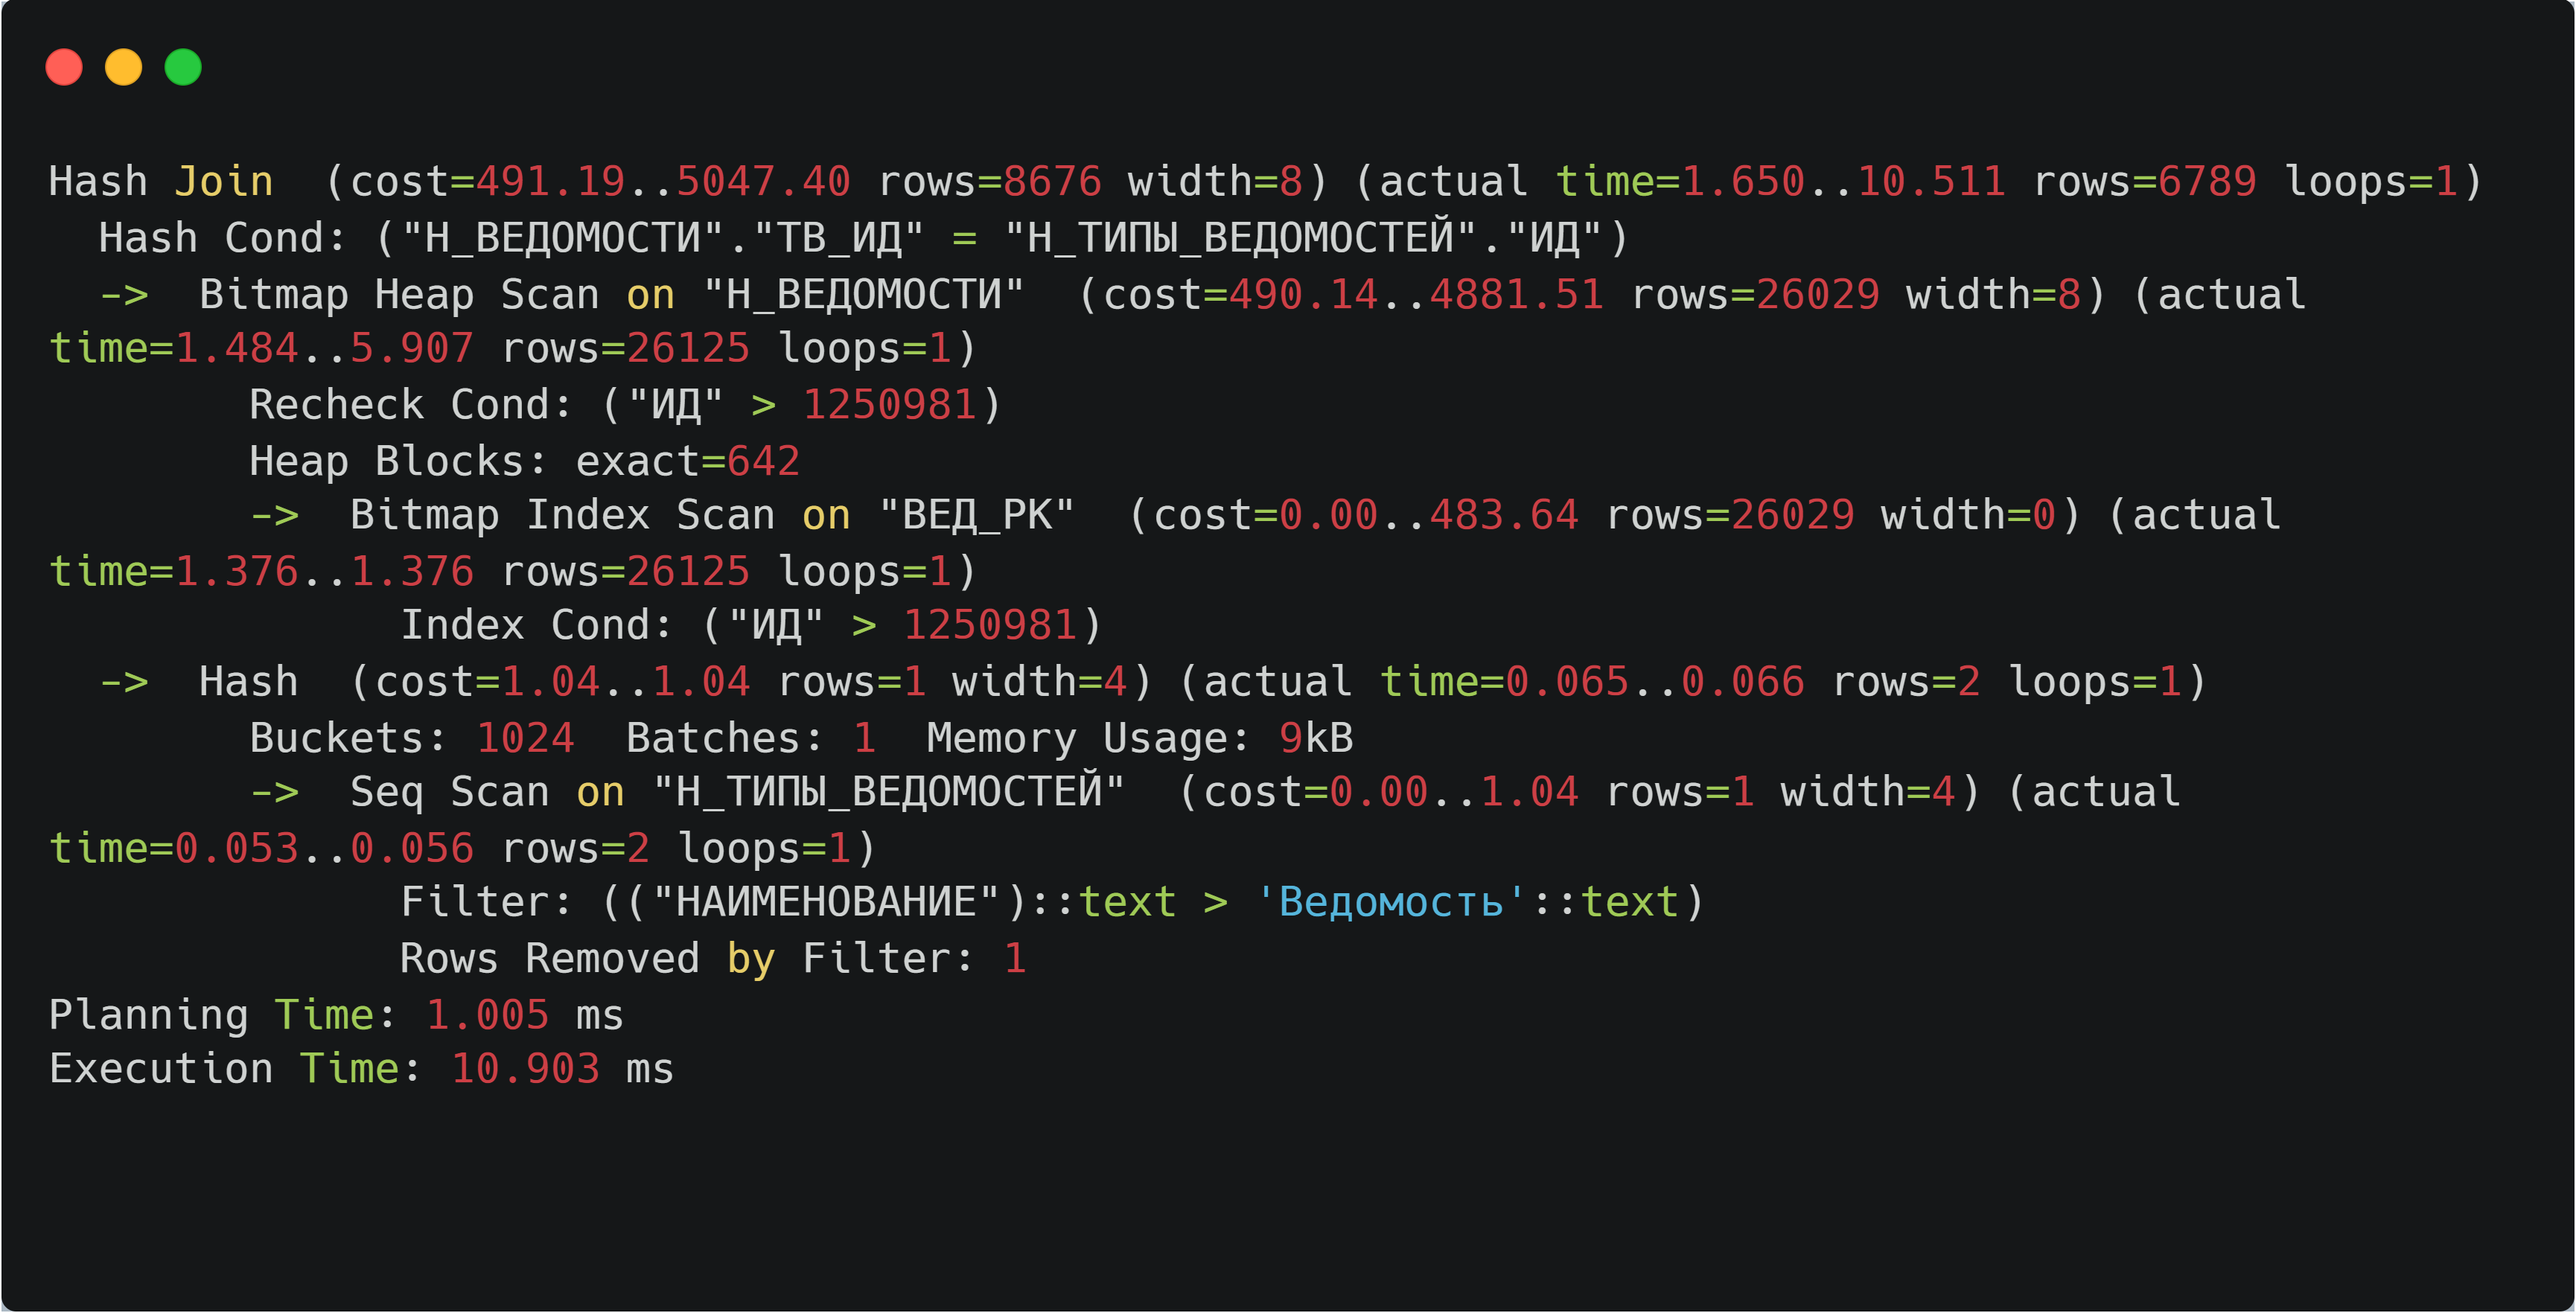
\includegraphics[width=\linewidth]{explain1}
	\newpage
	\section{Вывод}
	При выполнении данной лабораторной работы я узнал понятие индексов в базах данных и как их использовать. Научился составлять планы и выбирать наиболее выгодный. Узнал про виды оптимизации соединения таблиц
\end{document}







